    { \footnotesize
    \begin{figure}
    \centering
    %
    \begin{subfigure}{.3\textwidth}
      \[
        %
        \begin{array}{l}
            \kw{whileOdd}(k) \triangleq \\
            \clabel{ \assign{i}{k} }^{0} ; \\
                \ewhile ~ \clabel{i > 0}^{1} ~ \edo ~ \\
                \qquad \Big(
                  \eif(\clabel{i \% 2 == 0 }^{2}, \\
                  \qquad \qquad \clabel{\assign{i}{i - 1}}^{3},\\
                  \qquad \qquad \clabel{\assign{i}{i - 3}}^{4});
                  \Big)
            \end{array}
        \]
    \end{subfigure}
    \begin{subfigure}{.3\textwidth}
        \begin{centering}
        \begin{tikzpicture}[scale=\textwidth/15cm,samples=200]
    \end{tikzpicture}
    \caption{}
    \end{centering}
    \end{subfigure}
    %
\begin{subfigure}{.4\textwidth}
                \begin{centering}
                    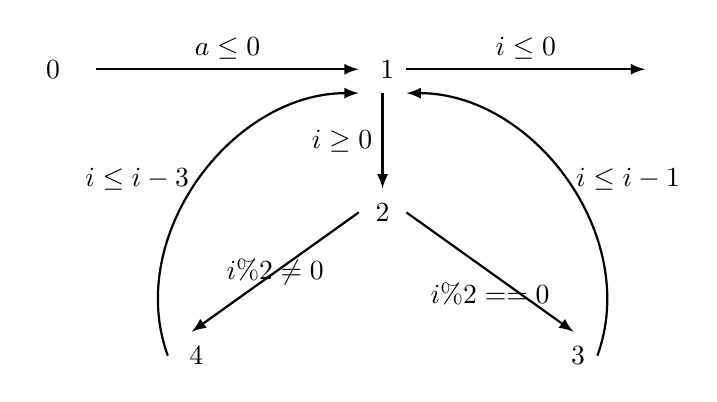
\begin{tikzpicture}[scale=\textwidth/20cm,samples=200]
                        \draw[] (-7, 10) circle (0pt) node{{ $0$}};
                        \draw[] (0, 10) circle (0pt) node{{ $1$}};
                        \draw[] (0, 7) circle (0pt) node{\textbf{$2$}};
                        \draw[] (4, 4) circle (0pt) node{{ $3$}};
                        % \draw[] (0, 1) circle (0pt) node{{ $4$}};
                        \draw[] (-4, 4) circle (0pt) node{{ $4$}};
                        % Counter Variables
                        \draw[] (6, 10) circle (0pt) node {\textbf{$\lex$}};
                        % \draw[] (6, 4) circle (0pt) node {{ $ex$}};
                        %
                        % Control Flow Edges:
                        \draw[ thick, -latex] (-6, 10)  -- node [above] {$a \leq 0$}(-0.5, 10);
                        \draw[ thick, -latex] (0, 9.5)  -- node [left] {$i \geq 0$} (0, 7.5) ;
                        \draw[ thick, -latex] (0.5, 7)  -- node [below] {$ i \% 2 == 0 $}  (4, 4.5);
                        \draw[ thick, -latex] (-4.5, 4)  to  [out=110,in=180]  node [left] {$i \leq i - 3$ }(-0.5, 9.5);
                        \draw[ thick, -latex] (4.5, 4)  to  [out=70,in=0]   node [right] {$i \leq i - 1$ }(0.5, 9.5);
                        \draw[ thick, -latex]  (-0.5, 7) -- node  {$i \% 2 \neq 0$}  (-4, 4.5) ;
                        \draw[ thick, -latex] (0.5, 10)  -- node [above] {$i \leq 0$}  (5.5, 10);
                        % \draw[ thick, -latex] (6, 6.5)  -- node [right] {$\top$} (6, 4.5) ;
                        \end{tikzpicture}
             \caption{}
                \end{centering}
                \end{subfigure}
\begin{subfigure}{.5\textwidth}    
    \begin{centering}
        $
        \begin{array}{l}
            0 \to 1; \\
    \rpchoose\{
        \eskip,\\
        \qquad \rprepeat(\rprepeat(2 \to 3 \to 1); 2 \to 4 \to 1),
        \\
        \qquad \rprepeat(\rprepeat(2 \to 4 \to 1); 2 \to 3 \to 1)
        \}; \\
        1 \to \lex
\end{array}
$
\caption{}
\end{centering}
\end{subfigure}
    \caption{
    (a) An example of multiple path while loop 
    (b) The Constraint Program
    (c) The Refined Program.}
        \label{fig:whileOdd}
    \end{figure}
    }

